%+++++++++++++++++++++++++++++++++++++++++++
\documentclass[conference]{IEEEtran}
%+++++++++++++++++++++++++++++++++++++++++++
% Added to commands
\input epsf
\usepackage{graphicx}
\usepackage{url}
\usepackage{subcaption}

%+++++++++++++++++++++++++++++++++++++++++++
% correct bad hyphenation here
\hyphenation{op-tical net-works semi-conduc-tor IEEEtran}
\begin{document}

%+++++++++++++++++++++++++++++++++++++++++++
% paper title
\title{\LARGE Network Analysis of 'MiBici' Public Bike Service in Guadalajara's Metropolitan Area}

\author{Henry Marie MONT (C311035) and Matteo MATONE (C40241) \\
University of Tartu, Department of Computer Science \\
Tartu, Estonia \\
\texttt{henry.marie.mont@ut.ee, matone@ut.ee}}

\maketitle

\begin{abstract}
This paper presents a comprehensive network analysis of the public shared bike service known as "MiBici" in Guadalajara's metropolitan area (ZMG) in Jalisco, Mexico, spanning from December 2014 to January 2024. We delve into the network structure, dynamics, and user behaviors of the "MiBici" system using a variety of advanced network analysis techniques. Through meticulous data preprocessing, network construction, and detailed analysis scripts, we uncover crucial insights into the spatial distribution of bike stations, traffic flows, user mobility patterns, and overall system efficiency. Our findings reveal the intricate connections and usage patterns within the network, highlighting peak usage times, popular routes, and station connectivity. Furthermore, we identify key factors that influence user behavior and trip duration, providing a deeper understanding of how the system is utilized. These insights contribute significantly to the broader understanding of public bike-sharing systems and offer valuable recommendations for improving service operations. Additionally, our study provides actionable information for urban planners and transportation managers, aiding in the development of more efficient and user-friendly bike-sharing systems. 
\end{abstract}

\IEEEoverridecommandlockouts

\begin{keywords}
Public bike-sharing, Network analysis, Complex network theory, Urban transportation, Mexico, Guadalajara.
\end{keywords}

\section{Introduction}
Public bike-sharing systems have witnessed a significant surge in popularity across urban areas worldwide, emerging as a sustainable and convenient mode of transportation. These systems, which provide users with access to bicycles for short trips, play a pivotal role in alleviating traffic congestion, reducing greenhouse gas emissions, and promoting healthier lifestyles. As urban populations continue to grow, the demand for efficient and eco-friendly transportation alternatives becomes increasingly critical. Public bike-sharing programs address this need by offering a practical solution that integrates seamlessly with other forms of public transport, thus enhancing the overall mobility ecosystem in cities.

The concept of bike-sharing is not entirely new; it has evolved over the decades, adapting to technological advancements and changing urban landscapes. Early iterations of bike-sharing systems often faced challenges related to theft, vandalism, and operational inefficiencies. However, modern systems have significantly improved through the incorporation of advanced technologies such as GPS tracking, mobile applications, and data analytics. These innovations have enhanced the user experience, making bike-sharing more reliable and accessible, while also providing operators with valuable data to optimize system performance.

Understanding the dynamics of public bike-sharing systems is essential for optimizing service operations and guiding urban planning efforts. This involves analyzing various aspects such as network structure, user behaviors, and system efficiency. Network structure pertains to the spatial arrangement of bike stations and the interconnections between them. A well-designed network can facilitate smooth and efficient movement of users across the city, ensuring that bikes are available where and when they are needed. User behavior analysis sheds light on how individuals interact with the system, including patterns in trip frequency, duration, and preferred routes. System efficiency encompasses the operational aspects, such as bike redistribution strategies, maintenance, and real-time demand management.

The growing body of literature on public bike-sharing systems highlights the importance of data-driven approaches in understanding and improving these systems. Researchers have employed complex network theory, graph analysis, and other data-driven methodologies to uncover intricate relationships within bike-sharing networks. For instance, studies have examined the spatial distribution of bike stations, identifying key factors that influence station usage and trip patterns. Other research has focused on the temporal dynamics of bike-sharing, exploring how usage varies by time of day, day of the week, and season.

In this paper, we focus on the network analysis of the "MiBici" public bike service in Guadalajara's metropolitan area (ZMG) in Jalisco, Mexico. Launched in December 2014, MiBici has grown to become a vital component of the city’s transportation infrastructure, providing residents and visitors with an eco-friendly and efficient means of travel. Guadalajara, being one of the largest cities in Mexico, faces typical urban challenges such as traffic congestion, air pollution, and limited public transportation options. The introduction of MiBici was aimed at addressing these issues, promoting sustainable urban mobility, and improving the quality of life for its citizens.

The MiBici system spans a wide geographic area, encompassing diverse neighborhoods with varying socio-economic characteristics. This diversity presents unique challenges and opportunities for analyzing the system's network structure and user behaviors. By exploring the spatial distribution of bike stations, traffic flows, and user mobility patterns, we aim to gain comprehensive insights into the functioning of the MiBici system and its implications for urban transportation in Guadalajara. Specifically, our analysis focuses on several key aspects:

\begin{itemize}
    \item \textbf{Spatial Distribution of Bike Stations:} Understanding the geographic layout of bike stations is crucial for assessing the accessibility and coverage of the bike-sharing network. We analyze the placement of stations in relation to key urban landmarks, residential areas, commercial districts, and public transportation hubs. This helps identify areas with high demand and potential gaps in service coverage.

    \item \textbf{Traffic Flows and Usage Patterns:} By examining the flow of bike trips between stations, we can identify major corridors of movement and peak usage times. This involves analyzing trip data to detect patterns such as the most frequently used routes, times of day with the highest activity, and seasonal variations in bike usage. Such insights are valuable for optimizing bike redistribution strategies and ensuring a balanced availability of bikes across the network.

    \item \textbf{User Mobility Patterns:} Understanding how users interact with the bike-sharing system provides valuable information on user preferences and behaviors. We investigate factors such as trip duration, trip frequency, and the demographic characteristics of users. This helps in identifying different user segments and tailoring services to meet their specific needs.

    \item \textbf{System Efficiency and Operational Challenges:} Efficient operation of a bike-sharing system involves managing the availability and condition of bikes, ensuring timely maintenance, and effectively redistributing bikes to meet demand. We analyze operational data to assess the performance of the MiBici system, identify bottlenecks, and propose strategies for improving operational efficiency.
\end{itemize}

The methodology employed in our analysis includes data preprocessing, network construction, and the application of various network analysis techniques. Data preprocessing involves cleaning and preparing the raw data to ensure accuracy and consistency. This step is critical given the large volume of data and the potential for errors or missing values. Network construction involves creating a directed and weighted graph representing the MiBici system, with bike stations as nodes and trips between stations as edges. The weight of each edge reflects the number of trips between the corresponding stations, providing a measure of the traffic flow.

Network analysis techniques are then applied to uncover insights into the structure and dynamics of the MiBici system. These techniques include measures of centrality to identify key stations within the network, community detection algorithms to uncover clusters of stations with high interconnectivity, and temporal analysis to explore how usage patterns change over time. Additionally, we employ visualization tools to create intuitive and informative representations of the network, facilitating the identification of patterns and trends.

\section{Related work}
The exploration of public bicycle systems through network analysis has garnered significant attention in recent literature, offering insights into system structure, dynamics, and user behaviors. Several studies have contributed to this domain by employing complex network theory, graph analysis, and data-driven approaches to understand the intricate relationships within bike-sharing systems.

Wei, Xu, and Ma \cite{wei2019exploring} demonstrated the applicability of complex network theory and shortest path analysis in characterizing the public bicycle network structure in Yixing, China. Their study highlighted the importance of network topology, spatial distribution, and traffic flows in understanding system functionality and proposed urban planning strategies for enhancing public bicycle transport.

Yao et al. \cite{yao2019analysis} focused on analyzing urban bike-sharing systems using real-time data from the Nanjing public bicycle system. Their study employed complex network methods to examine station relationships, revealing geographical divisions in bike demand areas and the influence of neighboring stations on usage patterns. Insights gained facilitated understanding of system dynamics and the fulfillment of diverse travel needs.

Dobrzyńska and Dobrzyński \cite{dobrzynska2017structure} conducted a comprehensive analysis of the BiKeR public bike-sharing system in Białystok, Poland, emphasizing the dynamics of network topology changes and station location choices. Their research underscored the specificity of bike-sharing networks and provided valuable insights for network modifications and decision-making processes.

Jurdak \cite{jurdak2013impact} investigated the impact of cost and network topology on urban mobility using data from public bicycle share systems in two U.S. cities. By characterizing user mobility and network properties, the study identified cost-sensitive trends and provided recommendations for dynamic pricing and incentive schemes to improve system management and planning.

Xiao et al. \cite{xiao2021demand} addressed the challenge of short-term demand prediction in public bike-sharing programs, proposing a spatio-temporal graph convolutional network (STGCN) approach. Their study demonstrated the effectiveness of STGCN in predicting picking up/returning demand, offering superior accuracy compared to traditional recurrent neural network (RNN)-based models.

Builes-Jaramillo and Lotero \cite{builes-jaramillo2022spatial} conducted spatial-temporal network analysis of the public bicycle sharing system in Medellín, Colombia. By employing exploratory data analysis and network theory approaches, they characterized user demographics, trip purposes, and system usage patterns. Their findings highlighted the need for inclusive planning strategies to address challenges such as female user engagement and infrastructure expansion aligned with city dynamics.

These studies collectively contribute to advancing knowledge on public bicycle systems, offering insights into network structure, dynamics, user behaviors, and planning strategies, which are instrumental in promoting sustainable urban transportation. By leveraging findings from these studies, the analysis of the MiBici system can benefit from best practices and lessons learned from diverse contexts, enabling informed decision-making and strategic interventions to optimize system performance and enhance user experience in Guadalajara's metropolitan area.

\section{Dataset}

\subsection{Source}
The dataset analyzed is sourced from Kaggle, representing the MiBici public bike service in Guadalajara's metropolitan area from December 2014 to January 2024. It includes 25,863,690 public bike trips and information on 372 bike stations.

\subsection{Data Description}
The dataset comprises the Nomenclature dataset detailing bike station locations and the MiBici dataset recording bike trips, including trip IDs, user demographics, start/end times, origin/destination station IDs, and trip duration.

\subsection{Data Preprocessing}
The raw dataset was pruned to 1/10th of its original size and exported as 'mibici\_compact.csv'. 'Nomenclature' dataset was filtered to remove inactive stations, and unnecessary columns were dropped. In the 'MiBici' dataset, datetime columns were converted, 'Duration' column was standardized, and additional temporal features were extracted.

\subsection{Constructing the Network}
A directed and weighted graph of the MiBici network was created. Nodes representing bike stations were added using 'nomenclature' dataset, and edges representing bike trips were derived from 'MiBici' dataset. The network was visualized with nodes positioned according to geographical coordinates (see Figure \ref{fig:side_by_side}).

\begin{figure}[htbp]
    \centering
    \begin{subfigure}[b]{0.20\textwidth}
        \centering
        \includegraphics[width=\textwidth]{images/urban-areas-covered-mibici.png}
        \caption{Map of the MiBici network}
        \label{fig:network}
    \end{subfigure}
    \hfill
    \begin{subfigure}[b]{0.20\textwidth}
        \centering
        \includegraphics[width=\textwidth]{images/mibici-network.png}
        \caption{Constructed network}
        \label{fig:map}
    \end{subfigure}
    \caption{Real network vs our network}
    \label{fig:side_by_side}
\end{figure}

\subsection{Descriptive Analysis of the network}
The network comprises 359 nodes and 37,031 edges, with an average path length of 1.81. It exhibits a single large connected component, a density of 0.29, high reciprocity (0.78), and a clustering coefficient of 0.68, indicating typical travel patterns and interconnectivity across the city.


\section{Methodology}

\begin{itemize}
    \item \textbf{Literature Review and Data Exploration:} The study begins with a literature review to understand existing research and identify relevant patterns. Simultaneously, exploratory data analysis (EDA) is conducted to unveil dataset characteristics.
    
    \item \textbf{Data Preprocessing:} After EDA, data is preprocessed to clean, standardize, and reduce its size for efficient processing.
    
    \item \textbf{Feature Selection:} Key features are selected based on insights from literature and EDA, focusing on meaningful attributes.
    
    \item \textbf{Graph Construction:} A graph is built using selected features, where stations are nodes and trips are edges, facilitating relationship analysis.
    
    \item \textbf{Exploratory Analysis:} Basic analysis is performed on the graph to understand its properties and guide further exploration.
    
    \item \textbf{Network Preprocessing:} Preprocessing ensures the integrity of network analysis by removing irrelevant nodes or edges.
    
    \item \textbf{Pattern Identification:} Exploratory techniques identify patterns, such as temporal variations and trends.
    
    \item \textbf{Network Property Analysis:} Key network properties are analyzed to understand their characteristics and dynamics.
    
    \item \textbf{Result Interpretation:} Findings are interpreted to draw conclusions and implications, providing a comprehensive understanding of the dataset (see Figure \ref{fig:flowchart}).
\end{itemize}

\begin{figure}
    \centering
    \includegraphics[width=0.75\linewidth]{images/Flowchart.png}
    \caption{Network analysis flowchart}
    \label{fig:flowchart}
\end{figure}

\section{Results}

\subsection{Temporal Evolution of Bike Stations}
Visualization of the bike stations' deployment over the years shows a gradual expansion of the network. The system had a slow start in 2014 and 2015, with limited activity. However, by 2016, the network became significantly more active, indicating increased adoption and utilization. During the initial years, most trips were concentrated in the city center, suggesting that peripheral stations were added in subsequent years. This observation aligns with historical data that indicates the network was launched in 2014 and expanded thereafter \cite{itdp2014}.

\subsection{Temporal Analysis of Bike Traffic}
The temporal evolution of bike traffic reveals consistent usage throughout the year, likely influenced by Mexico's generally warm climate and the absence of extreme seasonal weather. Monthly average weights vary slightly, with minor peaks and troughs. Further analysis shows that bike usage is lower on weekends compared to weekdays, suggesting that the primary use of the bike-sharing system is for commuting rather than leisure (see Figure \ref{fig:mibici-temporal-analysis}).

\begin{figure}[htbp]
    \centering
    \begin{subfigure}[b]{0.20\textwidth}
        \centering
        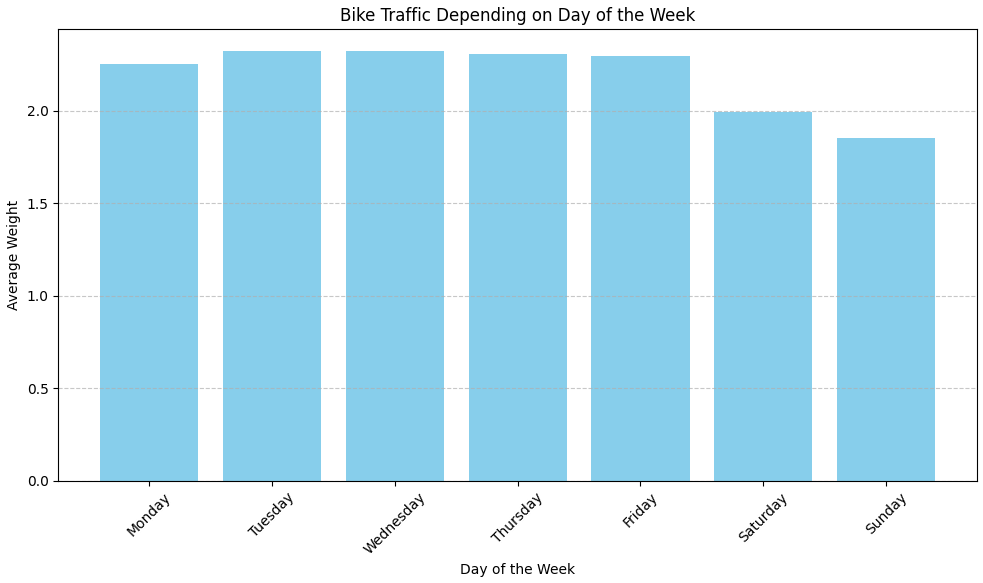
\includegraphics[width=\textwidth]{images/mibici-weekday.png}
        \caption{Daily traffic}
        \label{fig:mibici-daily}
    \end{subfigure}
    \hfill
    \begin{subfigure}[b]{0.20\textwidth}
        \centering
        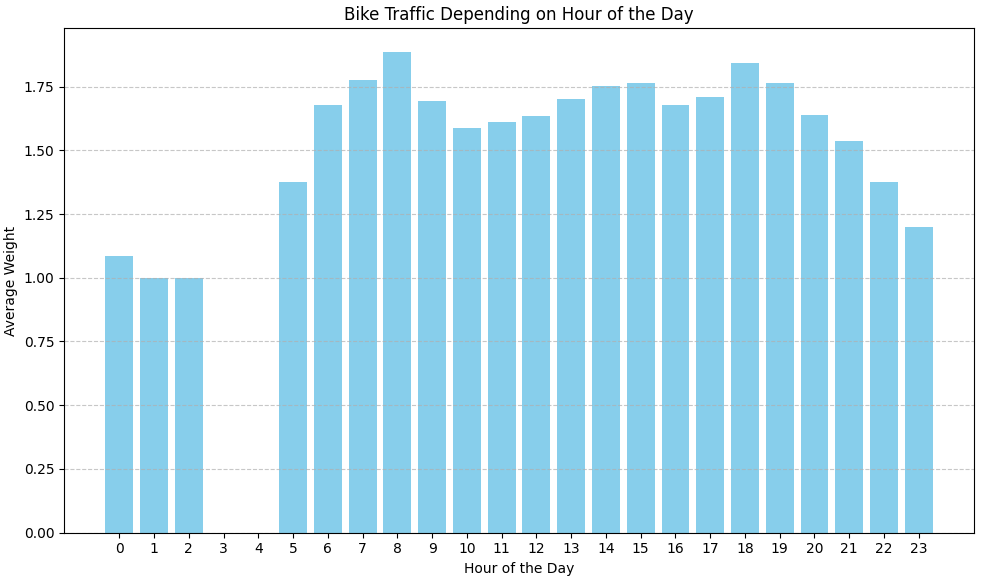
\includegraphics[width=\textwidth]{images/mibici-hour.png}
        \caption{Hourly traffic}
        \label{fig:mibici-hourly}
    \end{subfigure}
    \caption{Daily and Hourly traffic}
    \label{fig:mibici-temporal-analysis}
\end{figure}

Hourly bike traffic analysis indicates peak usage during morning (7-9 AM) and evening (5-7 PM) commute times, with minimal activity between midnight and 5 AM. This is consistent with the system's operational hours, as stations are closed from midnight to 6 AM \cite{mibici2023}. Limited activity during closed hours likely reflects maintenance and bike redistribution efforts by network employees.

\subsection{Network Centrality}
Centrality analysis highlights the most important bike stations, predominantly located in the city center along major axes. These central stations exhibit higher usage due to their strategic locations, facilitating frequent intra-city travel. Peripheral stations, by contrast, are primarily used during commute times, reflecting their role in connecting residential areas to the city center (see Figure \ref{fig:side_by_side}).

\begin{figure}[htbp]
    \centering
    \begin{subfigure}[b]{0.20\textwidth}
        \centering
        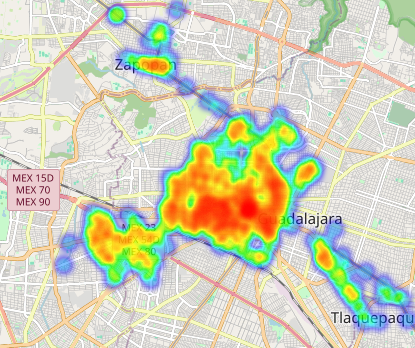
\includegraphics[width=\textwidth]{images/guadalajara_all_stations.png}
        \caption{Map of all stations}
        \label{fig:network}
    \end{subfigure}
    \hfill
    \begin{subfigure}[b]{0.20\textwidth}
        \centering
        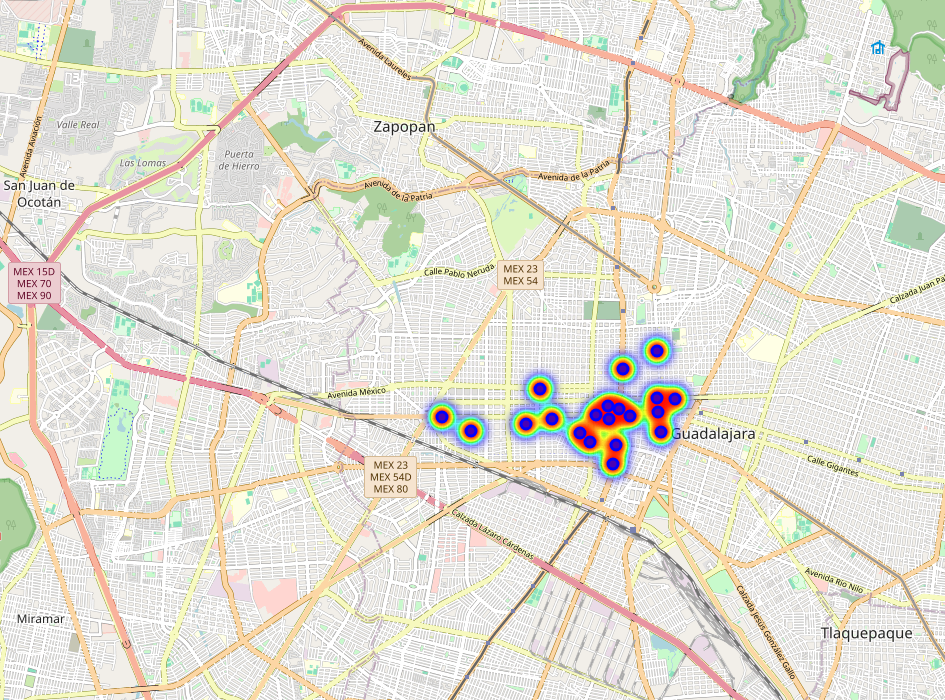
\includegraphics[width=\textwidth]{images/guadalajara_central_stations.png}
        \caption{Map of central stations}
        \label{fig:map}
    \end{subfigure}
    \caption{All stations vs Central stations}
    \label{fig:side_by_side}
\end{figure}

\subsection{Community Detection}
Community detection reveals five distinct communities within the network, forming a triangular spatial distribution with vertices representing peripheral areas. Two central communities are identified within the city center, indicating high interconnectivity and localized travel within these areas. The peripheral communities are linked to the outer edges of the city center, reflecting daily commuting patterns between residential and work areas. The lack of cross-city center travel suggests localized movement within specific areas of the city center, supported by public transportation or walking (see Figure \ref{fig:mibici-communinities}).

\begin{figure}
    \centering
    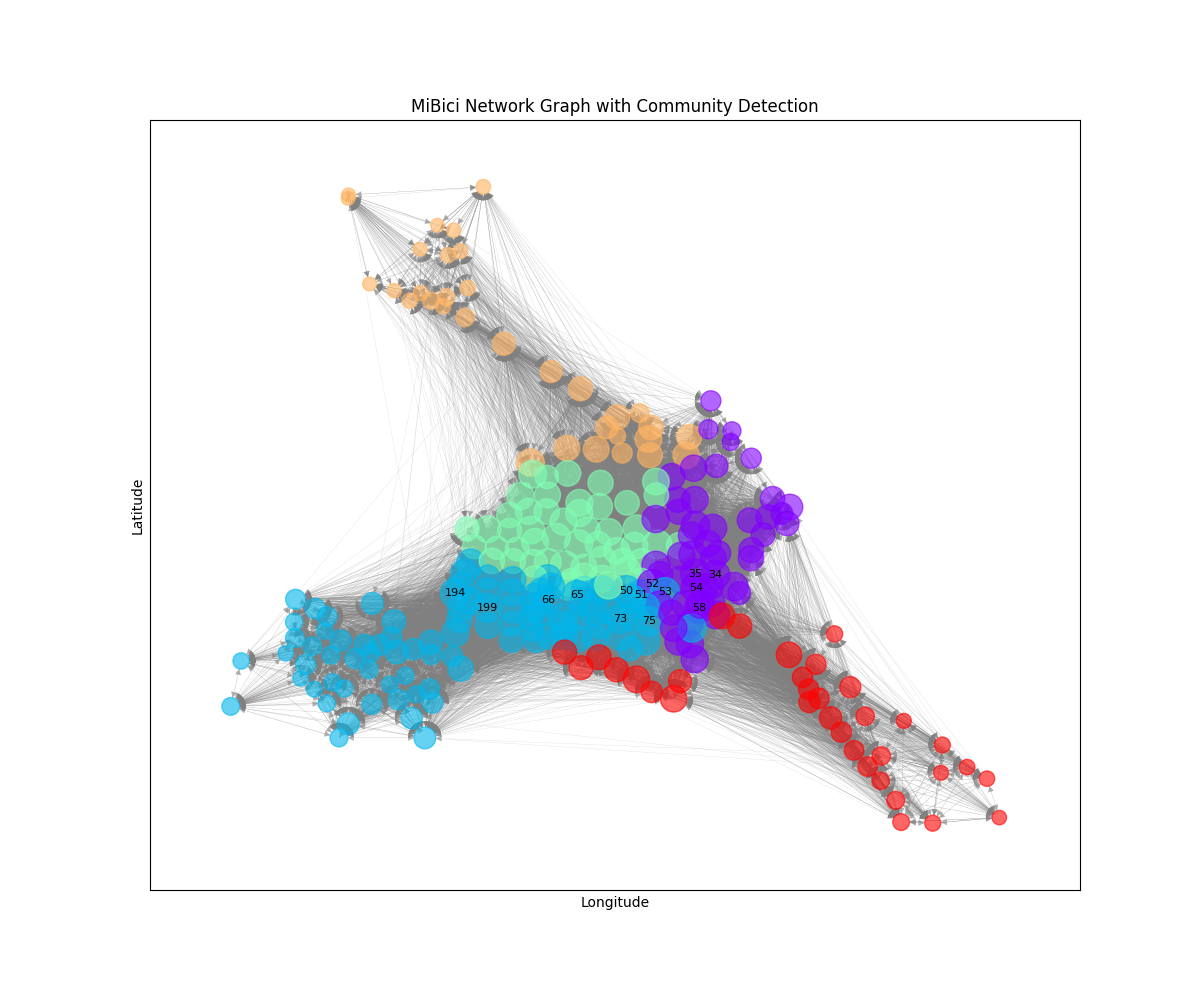
\includegraphics[width=0.5\linewidth]{images/mibici-network-communities.png}
    \caption{MiBici Network Communities}
    \label{fig:mibici-communinities}
\end{figure}


\section{Conclusion}

The network analysis of the "MiBici" public bike-sharing system in Guadalajara's metropolitan area reveals critical insights into its structure, user behavior, and operational efficiency over nearly a decade. Our comprehensive study highlights several key findings that can inform future enhancements to bike-sharing services and urban mobility strategies.

Firstly, the spatial distribution of bike stations and their connectivity patterns reveal a well-integrated network, with a central hub in the city center and peripheral nodes facilitating commute between residential and commercial areas. This structure supports efficient intra-city travel, particularly during peak commuting hours, as indicated by the observed traffic flows and usage patterns.

Temporal analysis underscores the role of "MiBici" in daily commutes, with pronounced activity peaks during morning and evening rush hours. This consistent usage pattern throughout the year, unaffected by seasonal weather changes, emphasizes the system's reliability and importance in Guadalajara's transportation landscape.

Centrality and community detection analyses further illuminate the network's dynamics. Central stations exhibit higher usage, reflecting their strategic locations, while peripheral stations connect residential zones to the city center. The identified communities within the network correspond to localized travel patterns, suggesting that users predominantly move within specific areas rather than across the entire city center. This insight is crucial for optimizing bike redistribution strategies and enhancing service availability.

\begin{thebibliography}{1}

\bibitem{wei2019exploring}
Wei, Sheng, Jiangang Xu, and Haitao Ma. “Exploring Public Bicycle Network Structure Based on Complex Network Theory and Shortest Path Analysis: The Public Bicycle System in Yixing, China.” \textit{Transportation Planning and Technology} 42, no. 3 (2019): 293–307. doi:10.1080/03081060.2019.1576385.

\bibitem{yao2019analysis}
Yao, Yi, Yifang Zhang, Lixin Tian, Nianxing Zhou, Zhilin Li, and Minggang Wang. 2019. "Analysis of Network Structure of Urban Bike-Sharing System: A Case Study Based on Real-Time Data of a Public Bicycle System" \textit{Sustainability} 11, no. 19: 5425. https://doi.org/10.3390/su11195425.

\bibitem{dobrzynska2017structure}
Dobrzyńska, Ewa, and Dobrzyński, Maciej. "Structure and dynamics of a public bike-sharing system. Case study of the public transport system in Białystok" \textit{Engineering Management in Production and Services} 8, no.4 (2017): 59-66. https://doi.org/10.1515/emj-2016-0033.

\bibitem{jurdak2013impact}
Jurdak, Raja. "The Impact of Cost and Network Topology on Urban Mobility: A Study of Public Bicycle Usage in 2 U.S. Cities." \textit{PLoS ONE} 8, no. 11 (2013): e79396. https://doi.org/10.1371/journal.pone.0079396.

\bibitem{xiao2021demand}
Xiao, G., Wang, R., Zhang, C. et al. Demand prediction for a public bike sharing program based on spatio-temporal graph convolutional networks. \textit{Multimed Tools Appl} 80, 22907–22925 (2021). https://doi.org/10.1007/s11042-020-08803-y.

\bibitem{builes-jaramillo2022spatial}
Builes-Jaramillo, Alejandro, and Laura Lotero. "Spatial-temporal network analysis of the public bicycle sharing system in Medellín, Colombia." \textit{Journal of Transport Geography} 105 (2022): 103460. https://doi.org/10.1016/j.jtrangeo.2022.103460.

\bibitem{torres2021sustainable}
Torres, Arturo, Ortega, Andrea, Sudmant, Andrew, \& Gouldson, Andy. (2021). Sustainable Mobility for Sustainable Cities: Lessons from Cycling Schemes in Mexico City and Guadalajara, Mexico.

\bibitem{quirarte2024mibici}
Quirarte, Sebastián. (2024). Over 9 Years of Real Public Bike Use Data - MiBici. Kaggle. \url{https://www.kaggle.com/datasets/sebastianquirarte/over-9-years-of-real-public-bike-use-data-mibici}

\bibitem{itdp2014}
MiBici Bike Share Arrives in Guadalajara, Mexico, December 08 2014, \url{https://itdp.org/2014/12/08/mibici-bike-share-arrives-guadalajara-mexico/}, accessed on May 27, 2024.

\bibitem{mibici2023}
About MIBICI, \url{https://www.mibici.net/en/about-mibici/}, accessed in 2024.

\end{thebibliography}

\section{Github}

The source code of the project can be viewed on Github at \url{https://github.com/monthenry/Network-Science-Project}.

\end{document}